\documentclass[10pt]{article}

\usepackage[table]{xcolor}% http://ctan.org/pkg/xcolor
\usepackage[english, spanish]{babel}
\usepackage[utf8]{inputenc}
\usepackage{indentfirst}
\usepackage{float} % Para ubicar imagenes en donde corresponden
\usepackage{graphicx}
\usepackage{amsmath}

\usepackage{titlesec}
\usepackage{booktabs}
\usepackage{amsfonts}

\usepackage{pgfgantt}
\setcounter{secnumdepth}{4}
\titleformat{\paragraph}{\normalfont\normalsize\bfseries}{\theparagraph}{1em}{}
\titlespacing*{\paragraph}{0pt}{3.25ex plus 1ex minus .2ex}{1.5ex plus .2ex}

\usepackage{fancyhdr}
	\lhead{}
	\chead{}
	\rhead{}
	\rfoot{\thepage}
	\cfoot{}
	\renewcommand{\headrulewidth}{0pt}
	\renewcommand{\footrulewidth}{0pt}
	\pagestyle{fancy}

%% Sets page size and margins
\usepackage[ a4paper, top=1.5cm, bottom=1.5cm, inner=1cm, outer=2cm, bindingoffset=2cm]{geometry}

\usepackage{caption}
\captionsetup[table]{name=Tabla}
\captionsetup[figure]{name=Figura}

\usepackage[backend=bibtex,style=numeric,maxcitenames=1,natbib=true,sorting=none]{biblatex} % Use the bibtex backend with the authoryear citation style (which resembles APA)
\addbibresource{bibs/references} % The filename of the bibliography
\usepackage[autostyle=true]{csquotes} % Required to generate language-dependent quotes in the bibliography

%Used to draw gantt charts, which I will use for the calendar.
%Let's define some awesome new ganttchart elements:


%----------------------------------------------------------------------------------------
%	TITLE PAGE
%----------------------------------------------------------------------------------------
\begin{document}
	\begin{center}
		\thispagestyle{fancy}
		{\Large\bfseries Universidad Católica \enquote{Nuestra Señora de la Asunción} \par}
			\vspace{2mm}
		{\Large\bfseries Proyecto Final de Ingeniería Informática\par}
	    		\vspace{2mm}

	   	Tema: Desarrollo de un sistema de gestión de programas de estudio orientado a resultados pedagógicos.
	    		\vspace{1mm}
	    
	    Alumno: Luis Fernando Villalba Vera
	    		\vspace{1mm}
	   	
	   	Tutor: Ing. Sebastián Ortíz
	    		\vspace{1mm}
	   	
	   	Co-Tutor: Ing. Wilfrido Inchaustti
        
	\end{center}


%----------------------------------------------------------------------------------------
%	 CONTENT - SECTIONS
%----------------------------------------------------------------------------------------

% Include the chapters of the thesis as separate files from the Chapters folder
% \renewcommand{\chaptername}{Capítulo}

\section{Introducción}

\subsection{Justificación}
Existe un consenso, tanto entre los empleadores como los funcionarios de gobierno, de que en los Estados Unidos se necesita un mayor número de estudiantes en nivel técnico y universitario que posean habilidades comprobadas\citep{kuh_knowing_2014}. Esto ha llevado a una gran presión sobre las instituciones educativas para que provean más y mejor evidencia de los logros del proceso educativo\citep{kuh_knowing_2014}. Para intentar llenar este vacío se ha creado la evaluación basada en competencias, la cual se enfoca en valorar las habilidades adquiridas por un estudiante en el proceso de un programa educativo\citep{cartwright2009student}.
 
De esta manera, las aplicaciones de evaluación académica basadas en competencias han adquirido mucha importancia en los últimos años\citep{barrio_minton_evaluating_2016}. En dichas aplicaciones se busca conocer información acerca de las fortalezas y debilidades del estudiante de una manera modular, en contraposición a los métodos cuantitativos de evaluación. Dichos aprendizajes y competencias son expresados por segmentos de estudios o actividades, mediante resultados esperados medibles a nivel institucional, de programa, grado, o de curso; expresados en calificaciones asociadas a habilidades específicas y no a módulos o cursos de un programa de estudio\citep{kuh_using_2015}. 
 
Para poder realizar una evaluación basada en competencias de un programa educativo, el mismo programa tiene que estar diseñado con esta perspectiva educativa: los programas de estudio e incluso los mismos cursos que lo conforman, tienen que estar diseñados con una perspectiva de orientación a competencias\citep{lalor_ensuring_2017}. La creación de un programa de estudio es una tarea colaborativa que involucra a un gran número de personas que proponen el diseño curricular, los cursos, los resultados esperados del programa. Cada uno de estos elementos debe pasar por un proceso iterativo de creación, revisión y aprobación que involucra a varios funcionarios, autoridades y profesores de las instituciones involucradas\citep{boyle_curriculum_2016}. 
 
En el ámbito de las aplicaciones académicas, si bien existen aplicaciones que abarcan el diseño y la publicación de planes de estudio por parte de los profesores o encargados de las universidades, además de su revisión y posterior aprobación por el comité curricular, no se ha encontrado durante el proceso de relevamiento de herramientas existentes una aplicación que integre todos estos elementos en un sistema de gestión de evaluaciones basadas en competencias\citep{curricunet_webpage}\citep{courseleaf_webpage}\citep{deca_webpage}.
 
En este caso de estudio\citep{runeson2012case} planteamos la posibilidad de crear un sistema de gestión de programas de estudio orientado a resultados pedagógicos y exploramos los desafíos tanto técnicos como de interacción humano computador asociados a dicho desarrollo.

\subsection{Objetivos}
\subsubsection{Objetivo general}
Diseñar una aplicación que permita integrar y estructurar tareas separadas de un sistema académico para una gestión de programas educativos orientados a resultados pedagógicos, que provea soporte a flujos de trabajo para sus diferentes etapas de aprobación.

\subsubsection{Objetivos específicos}
  \begin{itemize}
    \item Realizar un relevamiento de los requerimientos y comparación de las herramientas existentes que aborden la problemática planteada.
    \item Realizar el proyecto en un marco de programación ágil, estimando y desarrollando la aplicación de acuerdo a las directrices brindadas por esta metodología.
    \item Validar la herramienta desarrollada con expertos del dominio principalmente y de manera preliminar con experiencias limitadas con los usuarios finales.
  \end{itemize}

\section{Marco Teórico}
% \subsection{Aplicaciones web} % (fold)
% La necesidad de ejecución de operaciones complejas de manera remota y portable, tales como el uso de software sin depender de la potencia del hardware del usuario, la disponibilidad de uso en múltiples plataformas, y muchas otras, han guiado al desarrollo y evolución de las aplicaciones web. En las ciencias de la computación, una aplicación web es un software con arquitectura cliente-servidor donde el cliente (o interfaz de usuario) corre en un navegador web\citep{net_app_architecture}.

% Los usuarios acceden a la aplicación utilizando un navegador web y no es necesario descargarse ningún tipo de software adicional, ya que la aplicación se ejecuta en el servidor. Para esclarecer el panorama, la lógica de la aplicación web se ejecuta remotamente, y el navegador web sólo se limita a la representación de los datos.

% La evolución de las aplicaciones web ha crecido tan vertiginosamente que además de ofrecer una multitud de servicios, mejoran la UX a través de interfaces gráficas e intuitivas para los usuarios\citep{myers_past_2009}.

% \subsection{Cloud computing}
% La computación en la nube es una metáfora para abastecimiento y consumición de recursos de infraestructura. El nivel de abstracción ofrecida por la nube puede variar de hardware virtual a complejos sistemas distribuidos, debido a que los recursos están disponibles a demanda en enormes cantidades y pagados por uso\citep{wittig_amazon_2016}. Casi toda solución de infraestructura remota es basada hoy día con esta tecnología.

% La infraestructura remota o nube puede ser manejada por una organización abierta para uso público, o puede ser privada, donde una nube que virtualiza y comparte la infraestructura con una sola organización o híbrida.

\subsection{Software as a service}
SaaS\footnote{de sus siglas en inglés, Software as a Service, que significa en español software como servicio.}, es un paradigma de entrega de software donde la misma se encuentra alojada por lo general en la nube y se entrega como servicio a través de Internet a un gran número de usuarios a través de un modelo de suscripción. Se trata de un modelo de entrega de negocio en el que tanto la aplicación y el alojamiento son gestionados y compartidos con varias empresas, que alquilan y utilizan los servicios de aplicaciones de forma centralizada\citep{gupta_software_2014}.

% El software como servicio es equivalente a servicios de proveedores externos que manejan todo mantenimiento, personalización, actualización y cobro para los servicios que su cliente utiliza de manera mensual o anual. El proveedor se encarga de ofrecer el software basado en un conjunto de códigos y datos definidos junto a las diferentes configuraciones para los diferentes clientes. Los suscriptores al servicio acceden a la aplicación con la sensación de que son los únicos usuarios de la aplicación. Sin embargo, los cambios de configuraciones como cambios de datos, flujo de trabajo, interfaz y el flujo de negocio son realizados de manera masiva y transparente para ellos\citep{kumar_cloud_2012}\citep{kang_web_2012}.

% También existen otras opciones como PaaS\footnote{de sus siglas en inglés, Platform as a Service, que significa en español plataforma como servicio.} e IaaS\footnote{de sus siglas en inglés, Infraestructure as a Service, que significa en español infraestructura como servicio.}.

\subsection{Competencias académicas y su evaluación}
La creciente profesionalización trajo al campo educativo elementos evaluativos tales como calidad, equidad, competitividad, eficiencia, y eficacia; junto con ellos surgieron las competencias, que pasaron a jugar papel importante en el contexto educativo. En la formación de profesionales, resalta la necesidad de reflexionar sobre los aprendizajes que se ofrecen en las instituciones educativas, las cuales deben servir al estudiante para ser útil a la sociedad, que es su entorno inmediato \citep{kuh_using_2015}. En otras palabras, la competencia es la capacidad de un buen desempeño en contextos complejos y auténticos. Se basa en la integración y activación de conocimientos, habilidades, destrezas, actitudes y valores.

De esa necesidad va surgiendo la idea de las evaluaciones orientadas a competencias. Cabe resaltar cómo se desenvuelve el aprendizaje basado en competencias usando aplicaciones como herramientas para la evaluación de estudiantes, mediante el análisis de los aportes que introduce la tecnología en este campo, que modifican significativamente las prácticas tradicionales\citep{carriveau_connecting_2016}.

% Uno de los factores de motivación relevantes para el aprendizaje es la evaluación. Cada actividad ofrece a los estudiantes la oportunidad de conocer cuáles son sus resultados de aprendizaje en lo que se refiere al \enquote{qué} se ha aprendido y al \enquote{cómo} habría podido hacerse. Cualquier proceso de evaluación debería ser diseñado teniendo en cuenta este principio básico.

% En un sistema de gestión de evaluaciones basado en competencias, los encargados hacen evaluaciones según las evidencias obtenidas de diversas actividades de aprendizaje, que definen si un estudiante alcanza o no los requisitos recogidos por un conjunto de indicadores en un determinado grado. Una evaluación por competencias asume que pueden establecerse indicadores posibles de alcanzar por los estudiantes, que diferentes actividades de evaluación pueden reflejar los mismos indicadores\citep{barrio_minton_evaluating_2016}.

% La evaluación por competencias ofrece nuevas oportunidades a los estudiantes al generar entornos significativos de aprendizaje que acercan sus experiencias académicas al mundo profesional, y donde pueden desarrollar una serie de capacidades integradas y orientadas a la acción, con el objetivo de ser capaces de resolver problemas prácticos o enfrentarse a situaciones cotidianas \citep{carriveau_connecting_2016}.

Hoy día existen herramientas que ayudan al alumno a potenciar su aprendizaje y algunas de ellas son los sistemas de gestión de aprendizajes y los sistemas de gestión de evaluaciones basadas en competencias.

\subsection{Sistemas de gestión de evaluación}
Un AMS es un sistema, generalmente basado en tecnologías web, que permite a la institución la recolección, el manejo, y reporte de datos relacionados a las evaluaciones, por lo general basadas en competencias, del estudiante. Los AMS basadas en competencias permiten a la institución y a los educadores listar sus competencias, guardar, y mantener datos para cada competencia, facilitar conexiones a competencias similares de la institución, y generar reportes\citep{cartwright2009student}.

% Varios sistemas comerciales existen; incluyendo Blackboard Learn, Campus Lab, eLumen, LiveText, TaskStream, TracDat/Webfolio, Waypoint Outcomes y WEAVEOnline. También existen otras desarrolladas por las propias instituciones para manejar sus datos de evaluaciones.

% Mientras que cada AMS tiene un conjunto diferente de capacidades, todas manejan, mantienen, y permiten generar reportes de los datos de las evaluaciones. Generalmente, teniendo como ejemplo los distintos sistemas, los AMS tienen una estructura jerárquica basada en unidades organizacionales (programas, departamentos, escuelas, colegios o la misma institución), por lo tanto, las metas y/o las competencias también se ven adaptadas a esta estructura.

% \subsection{Programas de estudio}
% En términos generales, se puede definir un programa de estudios como una herramienta educativa que regula y ordena el proceso de enseñanza-aprendizaje a desarrollar en una unidad de aprendizaje determinada, orientando las actividades que profesor y alumno han de llevar a cabo para el logro de los objetivos planteados en dicha unidad, en relación con los objetivos del plan de estudios, de tal manera que el egresado concluya su carrera con el perfil deseado. En pocas palabras, es un esquema organizado de los contenidos situados dentro de una determinada unidad de aprendizaje\citep{lalor_ensuring_2017}.

% El termino \enquote{unidad de aprendizaje} sustituye al de \enquote{asignatura} o \enquote{materia} que evocan los tradicionales cursos unidisciplinarios, generalmente teóricos y sobrecargados de información. Un programa resume las características de la unidad de aprendizaje, su contenido mínimo obligatorio, y sus objetivos, principalmente.

% En la primera etapa de diseño curricular, se requiere la elaboración de la propuesta de los programas para su aprobación de parte de las autoridades con la colaboración de las academias y, de ser necesario, con la asesoría de externos de la unidad académica.

\subsection{Sistemas de gestión curricular}
Un CMS \footnote{de sus siglas en inglés, Curriculum Management System, que significa sistema de gestión curricular} es un aplicación automatizada que apoya todo el proceso curricular, desde la planificación hasta la implementación y evaluación. Posee una interfaz única y cohesiva en línea que permite proponer, crear, evaluar, revisar, aprobar y aplicar cursos, programas y competencias.

Curriculum es una mezcla sofisticada de estrategias educativas, contenido del curso, resultados de aprendizaje, experiencias educativas y evaluación\citep{harden2001amee}. Esta visión amplia de un CMS se deriva del ambiente actual de educación elemental y secundaria que es impulsado por los estándares de contenido de cursos obligatorios federales y estatales, y la necesidad de auditorías continuas de currículo\citep{west2000technology}.

En los enfoques actuales del desarrollo de Curriculum por lo general gira en torno a los comités curriculares. Dichos aspectos, sin embargo, sólo se consideran en un alto nivel de abstracción basado en la comprensión tácita de los miembros del comité sobre la disciplina.


\subsection{Metodología Ágil de desarrollo de software}
La metodología Ágil envuelve un enfoque para la toma de decisiones en los proyectos de software, que se refiere a métodos de ingeniería del software basados en el desarrollo iterativo e incremental, donde los requisitos y soluciones evolucionan con el tiempo según la necesidad del proyecto\citep{davis_agile_2015}. Los métodos tradicionales, como Waterfall, pretenden ser capaces de modelar completamente el dominio del problema de entrada y luego esperar que se produzcan pequeños cambios (o inclusive ninguno)\citep{davis_agile_2015}. Los métodos ágiles asumen que el cambio es inevitable, por lo que abordan el desarrollo de software de tal manera a facilitar la adaptación de los nuevos requisitos mientras vayan surgiendo.

% Las metodologías ágiles, en comparación a otras metodologías de desarrollo, ofrecen un modelo de diseño flexible que fomenta al desarrollo evolutivo. Los desarrolladores trabajan en pequeños módulos cada vez y la retroalimentación proveída por el cliente ocurre simultáneamente en el desarrollo. Además, la metodología puede ser bastante útil en situaciones donde los objetivos finales del proyecto no están claramente definidos donde los requisitos del cliente se clarificarán gradualmente a medida que el proyecto avance.

% El uso de la metodología ágil como método de entregas de las características del módulo entra como requisito no funcional.

\subsubsection{Historias de usuario}
Las historias de usuario conforman la parte central de muchas metodologías de desarrollo ágil, tales como XP\footnote{de sus siglas en inglés, eXtreme Programming, que significa en español programación extrema}, Scrum, entre otras. Estas definen lo que se debe construir en el proyecto de software, tienen una prioridad asociada definida por el cliente de manera a indicar cuales son las más importantes para el resultado final. Son divididas en tareas y su tiempo es estimado por los desarrolladores.

% Por lo general, se espera que una estimación de tiempo de cada historia de usuario se sitúe entre horas y el tiempo máximo de iteración. Estimaciones superiores a este tiempo máximo son indicativas de que la historia es muy compleja y debe ser dividida en varias historias.

% Una historia de usuario es una representación de un requisito escrito en una o dos frases utilizando el lenguaje común del usuario\citep{davis_agile_2015}. Ellas son utilizadas para la especificación de requisitos acompañadas de las discusiones con aquellos y las pruebas de validación.

% Cada historia de usuario debe ser limitada. La metodología estipula que las mismas deben ser escritas por los clientes. Son una forma rápida de administrar los requisitos sin tener que elaborar gran cantidad de documentos formales y sin requerir de mucho tiempo para administrarlos.

% Las historias de usuario deben ser:
% \begin{itemize}
%     \item \textbf{Independientes:} de ser necesario, combinar las historias dependientes o buscar otra forma de dividir las historias de manera que resulten independientes.
%     \item \textbf{Negociables:} la historia en sí misma no es lo suficientemente explicita para considerarse un contrato, la discusión con los usuarios debe permitir esclarecerse y éste debe dejarse explicito bajo la forma de pruebas de validación.
%     \item \textbf{Valoradas:} Los intereses de los clientes y de los usuarios no siempre coinciden, pero en todo caso, cada historia debe ser más importante para los clientes que para el desarrollador.
%     \item \textbf{Pequeñas:} las historias grandes son difíciles de estimar e imponen restricciones sobre la planificación de un desarrollo iterativo. Generalmente se recomienda la consolidación de historias muy cortas en una sola historia.
%     \item \textbf{Estimables:} las historias completas en requerimientos de parte del equipo de desarrollo y de parte del cliente son estimables. Y por lo tanto, el equipo debe estar cómodo de puntuar las historias de usuario.
%     \item \textbf{Verificables:} las historias de usuario cubren requerimientos funcionales, por lo generalmente son verificables. Cuando sea posible, la verificación debe automatizarse, de manera que pueda ser verificada en cada entrega del proyecto.
% \end{itemize}

% Las iniciales de estas características, con sus nombres en inglés, forman la palabra INVEST, que significa “inversión”. Es porque toda historia de usuario, si se construye bien, es una inversión.

% Al momento de implementar las historias, los desarrolladores deben tener la posibilidad de discutirlas con los clientes. El estilo sucinto de las historias podría dificultar su interpretación, podría requerir conocimientos de base sobre el modelo, o podría haber cambiado desde que fue escrita.

% Cada historia de usuario debe tener en algún momento pruebas de validación asociadas, lo que permitirá al desarrollador, y más tarde al cliente, verificar si la historia ha sido completada. Como no se dispone de una formulación de requisitos precisa, la ausencia de pruebas de validación concertadas abre la posibilidad de discusiones largas y no constructivas al momento de la entrega del producto.

\subsubsection{Épicas}
Una épica es esencialmente una historia de usuario de un tamaño mucho mayor, siempre superior al tiempo de iteración máximo, y tiene como propósito el de asociar historias de usuario individuales relacionadas con un propósito de más alto nivel que cumplir. La misma es, por lo general, muy grande para que un equipo del proyecto pueda trabajar directamente sin partir en diversas historias de usuario\citep{cobb2015project}.

% El uso de las épicas en proyectos de gran tamaño ayuda a organizar tareas complejas en un tipo de estructura para que la interrelación de historias de usuario esté bien entendida. Por lo tanto, el diseño de épicas en el proceso de desarrollo es fundamental antes de comenzar cualquier proyecto.

\subsection{Interacción humano-computador}
En HCI definen la funcionalidad y la usabilidad de los sistemas que se desarrollan, donde la funcionalidad de un sistema es definida por un conjunto de acciones o servicios que son proveídas a los usuarios, sin embargo, el valor de la funcionalidad es verificada cuando es eficientemente utilizada por el usuario\citep{shneiderman_designing_2010}. La usabilidad de un sistema con cierta funcionalidad es el rango y grado por el cual el mismo puede ser utilizada de manera eficiente y adecuada para cumplir ciertas metas para ciertos usuarios. La eficiencia de un sistema es alcanzada cuando se cumple un balance entre la usabilidad y la funcionalidad\citep{nielsen_usability_2010}.

HCI es un diseño que debe producir un ajuste entre el usuario, la máquina y los servicios requeridos con el fin de lograr un balance óptimo entre la calidad y la eficiencia de los servicios.

La definición de la estrategia de UI\footnote{de sus siglas en inglés, User Interface, que significa en español experiencia de usuario.} es importante para una mejor usabilidad del sistema, donde este proceso debería comenzar antes que el diseño y desarrollo de las aplicaciones. Es la visión de una solución que necesite ser verificado con potenciales usuarios que prueben que necesite el mercado\citep{levy_ux_2015}.


\section{Estado del arte}
Una investigación para comprobar otros proyectos o productos con las mismas características propuestas, buscando innovación para el mercado es expuesta en la tabla \ref{relacion-sistemas}.

\begin{table}[H]
\centering
\begin{tabular}{lllccl}
\toprule
\multicolumn{3}{l}{Características}                                                & CurricUNET                       & CourseLeaf            & DECA         \\
\midrule
\multicolumn{3}{l}{Creación y versionamiento de competencias.}                     &                                  &                       &              \\
\multicolumn{3}{l}{Creación y versionamiento de cursos.}                           & $\checkmark$                     & $\checkmark$          & $\checkmark$ \\
\multicolumn{3}{l}{Creación y versionamiento de programas de estudio.}             & $\checkmark$                     & $\checkmark$          &              \\
\multicolumn{3}{l}{Cumple los Estándares de códigos de California.} 			   & $\checkmark$                     &                       &              \\
\multicolumn{3}{l}{Historial de versiones de competencias.}     			       & 			                      & 		              &  			 \\
\multicolumn{3}{l}{Historial de versiones de cursos.}     			               & $\checkmark$                     & $\checkmark$          & $\checkmark$ \\
\multicolumn{3}{l}{Historial de versiones de programas de estudio.}     		   & $\checkmark$                     &  			          & 			 \\
\multicolumn{3}{l}{Reporte de Comparación entre versiones de cursos.}              & $\checkmark$                     &                       & $\checkmark$ \\
\multicolumn{3}{l}{Soporta competencias de aprendizaje del estudiante.}            &                      			  &                       &              \\
\multicolumn{3}{l}{Plantilla de flujo de trabajo customizable.}                    & $\checkmark$                     &                       &              \\
\multicolumn{3}{l}{Permite asignar roles evaluadores en la aplicación.}            & $\checkmark$                     & $\checkmark$          &              \\
\multicolumn{3}{l}{Permite asignar usuarios como colaboradores.}                   & $\checkmark$                     &                       &              \\
\multicolumn{3}{l}{Sistema de alertas para colaboradores y evaluadores.}           & $\checkmark$                     & $\checkmark$          &              \\
\multicolumn{3}{l}{Buzón de entrada para colaboradores y autoridades.} 			   & $\checkmark$                     &                       & $\checkmark$ \\
\multicolumn{3}{l}{Soporte de correlatividades entre cursos.}                      & $\checkmark$ 					  &						  &              \\
\multicolumn{3}{l}{Incluye un catálogo de cursos.}                   		   	   & $\checkmark$					  &	$\checkmark$		  & $\checkmark$ \\
\multicolumn{3}{l}{Incluye un catálogo de programas de estudio.}                   & $\checkmark$					  &	            		  &              \\
\multicolumn{3}{l}{Incluye un catálogo de competencias.}                   	       & 								  &						  & 			 \\
\multicolumn{3}{l}{UX intuitiva y efectiva.}     			   					   &                                  & $\checkmark$          & $\checkmark$ \\
\bottomrule
\end{tabular}
\caption{Relación entre sistemas de gestión curricular.}
\label{relacion-sistemas}
\end{table}

En la actualidad existen aplicaciones web que son capaces de generar solicitudes de creación de planes de estudio mediante formularios. Entre ellas se encuentra CurricUNET, que es la aplicación que abarca gran parte de las necesidades de las universidades de California pero no cuenta con una manera de gestionar competencias o capacidad de integrarse a un AMS basado en competencias.

El análisis hecho por las herramientas fue una investigación de campo y entrevistas con los usuarios.

\subsection{CurricUNET}
CurricUNET es una aplicación web diseñada para automatizar la emisión y aprobación del plan de estudios emitido por profesores y/o encargados de universidades norteamericanas; que incluyen programas, cursos y competencias\citep{curricunet_webpage}.

En la misma se desarrollan propuestas de cursos y programas de estudio mediante formularios de la aplicación, con el objetivo de reemplazar solicitudes en papel que universidades utilizaban para emitir propuestas. Además, ofrece almacenamiento e información de plan de estudios históricos, activos y propuestos.

Todas las entradas, revisiones y reportes son accedidas por la web desde los navegadores. Posee un sistema de notificaciones integrado que permite al usuario un mejor seguimiento del progreso de las propuestas y cursos en revisión. Además, dispone de un control de versionamiento de cursos, planes de estudio y competencias.

Los usuarios del sistema pueden acceder a los reportes e historial de versiones de sus cursos y planes de estudio por lo que ayuda a una mejora continua del programa universitario.

\subsection{CourseLeaf}
El módulo de Curriculum de CourseLeaf es una solución de gestión basada en la web, mejorando los procesos de profesores y del comité de Curriculum de al menos 70 instituciones\citep{courseleaf_webpage}.

Cuando el módulo de Curriculum de CourseLeaf se combina con su módulo de catálogo, colegios y universidades son capaces de gestionar y realizar un seguimiento de la información del programa, desde la propuesta hasta publicar en una aplicación integrada con facilidad.

El software proporciona la generación de flujo de trabajo automático, notificaciones automáticas. Además, identifica todos los cursos, programas y departamentos que se ven afectados por los cambios propuestos en el inicio del proceso de propuesta y puede ayudar en la actualización con los cambios completados. El módulo de Curriculum de CourseLeaf se puede implementar con o sin su catálogo de Cursos.

\subsection{DECA: Curriculum Navigator}
DECA ofrece, mediante su módulo de Curriculum Navigator, una solución de desarrollo y administración de Curriculum\citep{deca_webpage}.

Cuando se utiliza como módulo integrado de su Catálogo, denominado como Catalog Navigator, proporciona una solución que les permite iniciar el camino de aprobación de alguna carrera de grado. Asesores y administradores, por otra parte, utilizan tanto Curriculum Navigator y Catalog Navigator para desarrollar y proporcionar datos públicamente del plan de estudios para sus estudiantes actuales y futuros.

\subsection{Relevancia del módulo curricular}
Frecuentemente, descrito como complejo e ineficaz, los métodos tradicionales basados en papel de gestión y diseño de programas de estudio proporcionan una visibilidad limitada, lo que resulta en una visión restringida de las etapas implicadas en la creación, modificación y aprobación de planes de estudio. Por lo tanto, se buscó eliminar esta complejidad al acelerar el desarrollo curricular y el proceso de aprobación.

En el flujo actual, una vez finalizado el proceso de diseño y revisión curricular de parte de las oficinas, se procede a publicar la nueva competencia, curso, o programa para que cada universidad tenga la información necesaria para ir cargando la misma en sus correspondientes sistemas. 

En el caso de las universidades comunitarias del estado de California, se utilizan los AMS para gestionar y evaluar las competencias de sus estudiantes. El proceso de registro de las nuevas entidades en los AMS es individual; eso quiere decir que un encargado del AMS tiene como trabajo el de cargar uno por uno las nuevas entidades aprobadas y publicadas por el comité curricular.

La importancia del módulo reside en la automatización de formularios y procesos que requieren la participación de personas ajenas al flujo de trabajo, para iniciar y validar propuestas de creación o revisión de cursos y programas. Luego, una vez que ha sido aprobada por el comité curricular se procede a la creación de las entidades de manera automática en el AMS.

Actualmente, hay alternativas que buscan solucionar la misma problemática pero no se ha encontrado durante el proceso de relevamiento de herramientas existentes una plataforma que pueda soportar el uso de competencias ni que pueda comunicarse con los sistemas de gestión de evaluaciones basadas en competencias.
\section{Caso de estudio}
\subsection{Diseño de la investigación}
El presente trabajo ilustra como caso de estudio la aplicación de la metodología ágil en la gestión de un proyecto de desarrollo de un módulo, integrado a un sistema de gestión y evaluación de competencias de una organización ubicada en los Estados Unidos. El trabajo realizado fue propuesto por la organización que brinda el sistema de gestión de competencias, donde el mismo sirve como base al módulo de gestión curricular a desarrollarse.

El caso refleja de manera práctica cómo se ha desenvuelto un proceso de desarrollo ágil en un diálogo con usuarios ubicados en diferentes localidades como parte del sistema de trabajo. En este proyecto los miembros ubicados en forma remota se encargan del diseño de las tareas, aquí llamadas historias de usuario, a realizarse, y de la validación de las características entregadas.

Debido a que los requisitos de la aplicación a desarrollarse se acordó desde un principio que se irían esclareciendo acorde se vayan completando las funcionalidades, se optó por la metodología ágil como técnica de gestión de desarrollo de software, puesto que era el enfoque más adecuado para poder encarar la problemática.

La observación participante de parte del investigador fue un paso inicial para el desarrollo del sistema en un nuevo equipo, donde se identifican y guían las relaciones con los informantes, lo ayuda a observar de manera embebida la organización y dinámica del equipo, y las prioridades de desarrollo. También, lo permite integrarse con los demás miembros del mismo y de esa manera le facilita el proceso de investigación, además de proveerle una cantidad de interrogantes a ser dilucidadas con los participantes \citep{erlandson_doing_1993}.

El primer paso fue adaptarse a los cambios y a la metodología de trabajo del equipo de desarrollo. Dicho equipo se constituyó luego de a una encuesta previa de capacidades de todos los desarrolladores de la empresa, donde cada uno colocó sus conocimientos en herramientas o en partes del sistema de gestión de competencias, para así poder aprovechar las virtudes de cada persona. Acto seguido se procedió al análisis de las herramientas a utilizarse para corroborar que cumplen con las exigencias del sistema a desarrollarse.

Entre algunas técnicas de recolección de información se utilizan las encuestas \citep{robson_real_2011}. Para este sistema un equipo en Estados Unidos utilizó la misma para proporcionar una visión general de los conocimientos generales del equipo de desarrollo.

Como caso de estudio con enfoque HCI\footnote{de sus siglas en inglés, Human-Computer Interaction, que significa en español interacción humano-computador.}, tuvo como meta la comprensión de problemas o situaciones mediante la interacción del ser humano con la computadora. Además, se buscó una documentación descriptiva del sistema y de su proceso de desarrollo, que apunta a la evolución del modelo propuesto durante el diseño de la misma, finalmente, se brinda y analiza evidencia de que la herramienta haya sido utilizada de manera exitosa mediante demostraciones a los usuarios o validaciones por parte del mismo \citep{lazar_research_2010}. 

Por lo tanto, el caso de estudio es con enfoque HCI y utiliza la observación participante como método principal de recolección de información.

\subsection{Dominio de la problemática}
El proyecto objetivo desarrollado utiliza como base una aplicación web AMS\footnote{de sus siglas en inglés, Assessment Management System, que significa en español sistema de gestión de evaluaciones.} que integra un módulo de gestión curricular a la misma. Los AMS son utilizados por las universidades en Estados Unidos para evaluar las competencias adquiridas de los estudiantes durante el proceso de su carrera o grado. También se busca la disponibilidad en dispositivos móviles. Los dispositivos inteligentes que van a poder utilizar la aplicación se definirán durante el proceso de desarrollo de la misma.

En las aplicaciones dirigidas al ambiente educativo, el hecho de utilizar nuevas tecnologías no asegura una mejor UX\footnote{de sus siglas en inglés, User eXperience, que significa en español experiencia de usuario.}, es por eso que utilizaremos durante el desarrollo de la aplicación técnicas de HCI \citep{lazar_research_2010}, encargadas de utilizar los patrones de diseño e interacción a seguir a la hora de construir cada uno de los componentes de la aplicación a ser desarrollada, y posteriormente validarlos.

Un requisito no funcional que forma parte de la infraestructura del caso de estudio es la utilización de la arquitectura SaaS\footnote{de sus siglas en inglés, Software as a Service, que significa en español software como servicio.}, ya que provee servicios bajo un modelo de pagos de suscripción por las diferentes características que la misma ofrece.

Durante el proceso de desarrollo, se definirán épicas a desarrollarse durante el periodo de diseño de la aplicación y las historias de usuario que están contenidas en las mismas, para que el equipo de desarrollo pueda entregar valor de negocio del módulo integrado en iteraciones cortas de dos semanas.

\subsection{Diseño curricular}
Para aquellas personas ajenas al entorno educativo, en específico aquellas que no forman parte del proceso de diseño curricular puede ser un tanto complejo el proceso de creación y revisión de material curricular en las instituciones. En la actualidad, un formulario de creación o revisión de competencias, cursos, y programas debe pasar por una serie de evaluadores que son los encargados de revisar y verificar que los datos sean válidos.

Hoy día el estado de California cuenta con un patrón de definición de cursos y programas donde la misma sirve como guía para el desarrollo de propuestas para material académico de las universidades. Dicho estándar además contiene una taxonomía de programas e indica cuál es el flujo para la revisión de las propuestas, donde todo es establecido en el PCAH\footnote{de sus siglas en inglés, Program and Course Approval Handbook, que significa en español manual de aprobación de cursos y programas.} \citep{brice_w_harris_program_2013}.

El flujo inicia con el profesor o encargado del curso o programa, una vez completado pasa por la mesa de recepción donde se verifica que cumpla con el estándar estatal para luego pasar por la oficina departamental y la oficina del decano para su revisión de contenido. Una vez revisado y con el visto bueno de ambas oficinas pasa por una última revisión por parte de la oficina curricular para ser registrada en los sistemas de gestión curricular.

Es un proceso que se hace con formularios en papel donde el profesor o encargado del curso o programa tiene que completar los campos requeridos para que el estado de California cuente al curso como válido. Dicho proceso tiene varias deficiencias:
\begin{itemize}
	\item La creación o revisión puede tomar meses debido a los formularios que son completados a mano y requieren de revisión de varias oficinas.
	\item Es un flujo de una sola dirección, eso quiere decir que si es que una de las oficinas rechaza el formulario debe volver a iniciar el flujo.
	\item Se puede producir cuellos de botella en los diferentes puntos de revisión.
\end{itemize}

Una vez ya registrado en los sistemas de gestión curricular es accesible de manera pública para el uso de las universidades del estado de California. De esta manera, si una institución académica posee un sistema de gestión de evaluaciones y quiere incluir los cursos o programas válidos para el estado tiene que ingresar los nuevos datos del sistema de gestión curricular uno a uno como se puede apreciar en la Figura \ref{after_creation}.

\begin{figure}[]
\centering
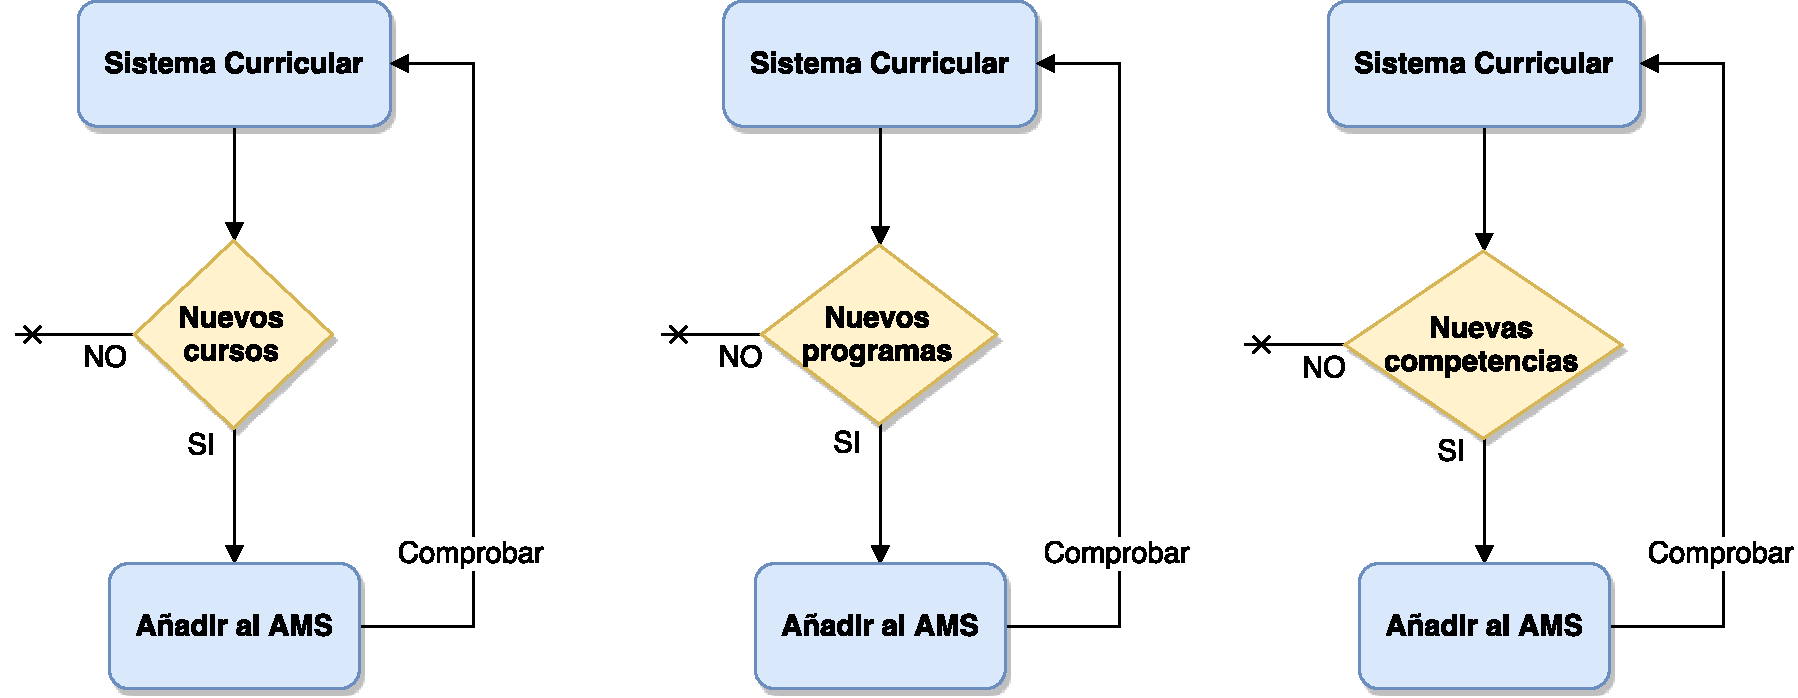
\includegraphics[width=125mm,scale=1]{img/after_creation}
\caption{Proceso de cargar datos desde el sistema curricular al AMS.}
  \label{after_creation}
\end{figure}
\section{Propuesta de trabajo} \label{propuesta_de_trabajo}
Una vez que los requerimientos iniciales han sido fijados y aclarados se busca la manera de automatizar los procesos, investigar tecnologías, y metodologías que ayuden al equipo de desarrollo para entregar funcionalidades de manera iterativa y evolutiva. Durante este proceso se diseñaron modelos donde se propone el módulo a ser desarrollado (Figura \ref{curriculum_model}) y se buscó unir procesos separados del diseño curricular con el flujo de agregar las competencias, cursos, y programas al AMS.

\begin{figure}[]
\centering
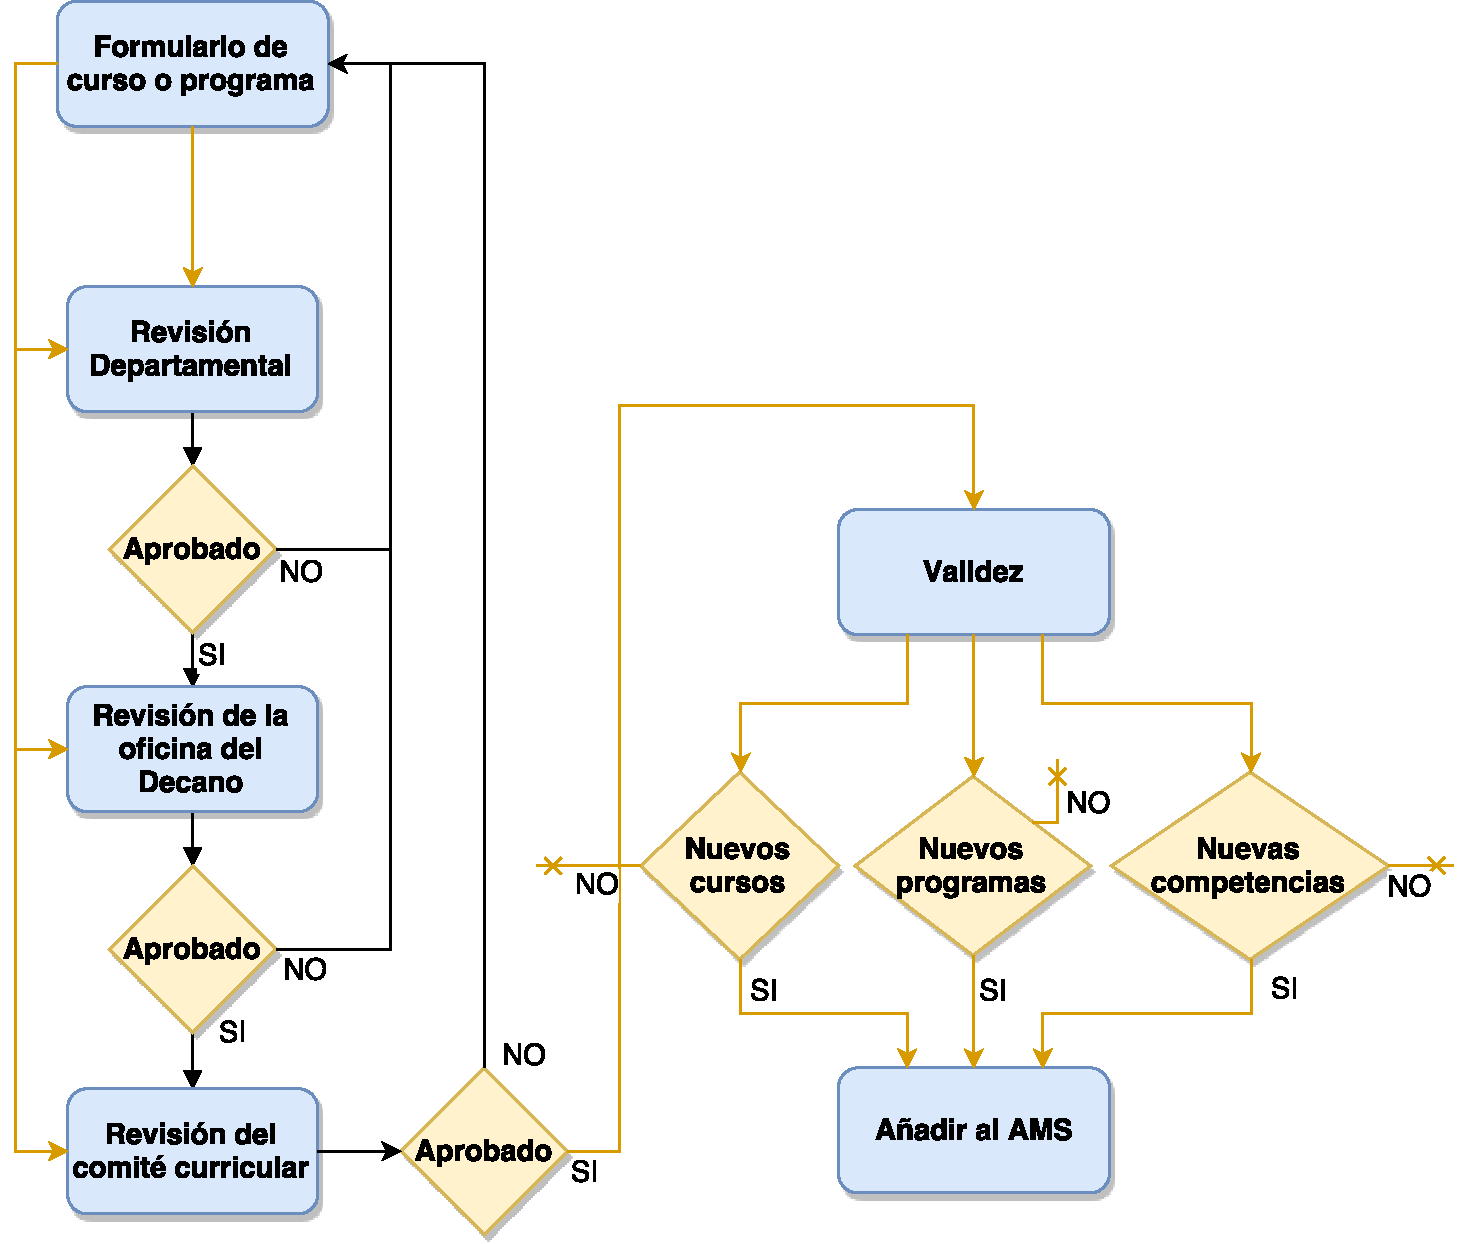
\includegraphics[scale=0.4]{img/curriculum_model}
\caption{Modelo propuesto del módulo curricular adherido a un sistema de gestión de evaluaciones basadas en competencias.}
  \label{curriculum_model}
\end{figure}

Con el uso de los formularios a papel, el encargado de curso o programa completa su formulario y lo entrega en la mesa de recepción, la misma se encarga de verificar que los datos completados sean válidos y cumpla con el estándar de creación de cursos y programas. 

El módulo buscó automatizar dicho proceso sacando la mesa de recepción como iniciador del flujo de validación mediante un formulario web. Además, se agrega un nuevo tipo de formulario para las competencias de las universidades comunitarias de California.

Luego, pasa por las oficinas del departamento, del decano, y del comité curricular para sus correspondientes revisiones. Si es que una de las oficinas rechaza el formulario debe volver al inicio con el encargado del mismo para volver a ser completado, y una vez terminado puede volver a pasar a la oficina que rechazó el formulario sin necesidad de volver a iniciar todo el proceso de corrección.

Y finalmente, una vez que el comité curricular acepta el formulario se procede a generar los nuevos cursos, programas, o competencias en el AMS. También, otro proceso automatizado por el módulo ya que dicha creación se desarrollaba de manera manual.

Además, se añade la funcionalidad de mensajes generados y notificaciones a los integrantes del flujo para evitar de esta manera los cuellos de botella con las revisiones, donde se notifican los pendientes y alertan trabajos en deuda.

\subsection{Modelo de arquitectura de módulo}

El proyecto final (figura \ref{arquitectura}) fue diseñado como módulo de un AMS utilizado en universidades del estado de California.

\begin{figure}[]
\centering
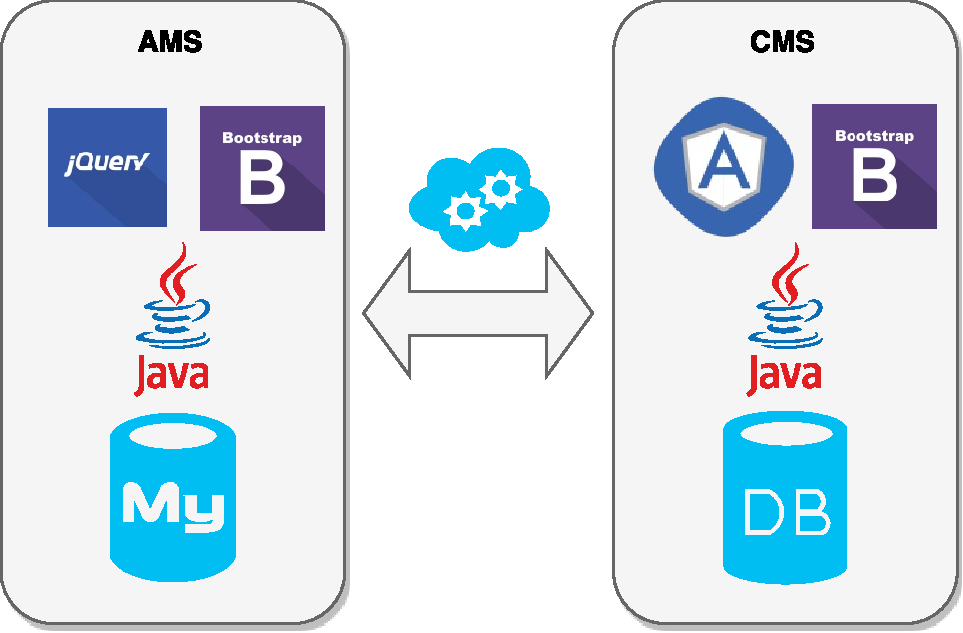
\includegraphics[scale=0.4]{img/arquitectura}
\caption{Arquitectura del módulo curricular.}
  \label{arquitectura}
\end{figure}

El AMS utilizado como base tiene una trayectoria de largos años de uso en varias universidades. Utiliza MySQL como motor de base de datos, Java como lenguaje de programación para la lógica de la aplicación y como conector a la base de datos se utiliza, y Bootstrap y JQuery para la interfaz de usuario. 

El proyecto final ha utilizado la misma base de datos, lenguaje de programación, y Bootstrap como requisitos no funcionales para el módulo curricular. Se optó cambiar JQuery a AngularJS debido a que al contar con un modelo MVC\footnote{de sus siglas en inglés, Model View Controler, que significa en español modelo vista controlador.} en la capa de presentación desde el comienzo resultó muy atractivo para acelerar el ritmo de trabajo y poder comenzar a implementar interfaces más complejas sin tener que preocuparse por las cuestiones más triviales que Angular maneja con directivas ya definidas como el uso de \enquote{data binding}, además, cuenta con una cantidad de documentación de parte de la comunidad que lo hacía aún más atractivo.
\section{Proceso de desarrollo}
El módulo como proyecto de desarrollo enfocado a la metodología Ágil se encuentra dividido en varias épicas para partir en las funcionalidades.

Una épica se encuentra dividida en varias historias de usuario, donde las historias de usuario tienen el propósito de entregar valores de negocio al cliente en un periodo establecido de 2 semanas como sprint. Estas historias de usuario pueden ser a la vez divididas buscando la simplicidad de las historias donde cada una debe seguir la práctica INVEST de la metodología Ágil.

Cada historia puede estar compuesta de tareas que tienen como propósito servir al desarrollador como recordatorio de algunas labores pendientes a la hora de desarrollar la historia. Cada tarea debía tener un encargado, pero no necesariamente una persona trabajando en dicha tarea.

% \begin{figure}[H]
% \centering
% 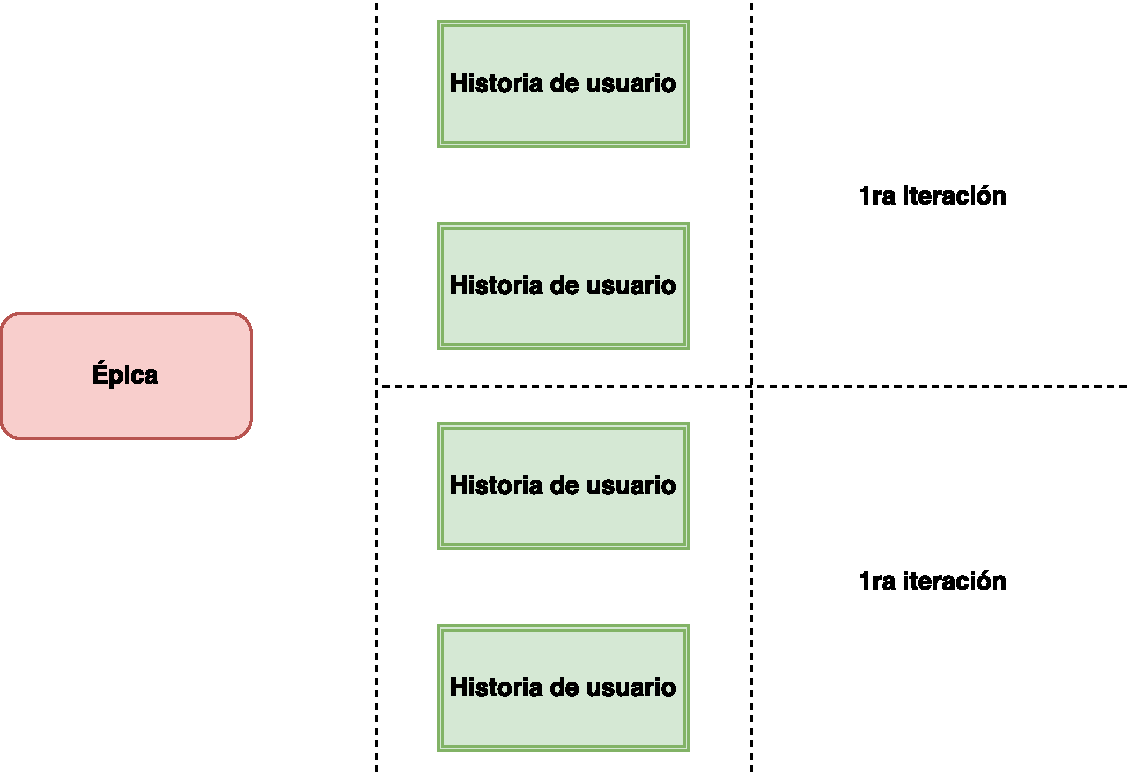
\includegraphics[width=125mm,scale=1]{Capitulos/PropuestadeSolucion/Imagenes/epic_diagram}
% \caption{Diagrama de definición de épicas en la metodología ágil}
%   \label{epic}
% \end{figure}

El PO\footnote{de sus siglas en inglés, Product Owner, que significa en español dueño del producto.} se encarga de la creación de épicas e historias de usuario, en caso de que la historia sea muy grande para terminar en un solo sprint o iteración se vuelve a partir en historias más pequeñas. 

Para el caso de estudio, cada sprint consta de 2 semanas de trabajo, donde los desarrolladores como equipo se comprometen a entregar cierto valor de negocio que ellos estiman poder terminar en dicho periodo. Sin embargo, en caso de que el equipo considere que la totalidad de historias no podrán ser entregadas antes de que termine el periodo se pasa al siguiente sprint o se achica la historia minimizando los criterios de aceptación y los restantes se agregan en otra historia de usuario para las siguientes iteraciones.

Cada equipo tiene un líder, donde cada líder tiene como rol ser la brecha que une al PO con los desarrolladores. El PO se reúne con el líder de cada equipo para verificar las prioridades de las historias de usuario que están pendientes en el backlog\footnote{Bolsa de historias de usuarios pendientes.}. 

Al inicio del diseño de la aplicación se llevará a cabo una serie de diseños de funcionalidad y usabilidad que llevar a la mejor experiencia de uso del módulo de gestión curricular, donde dichos diseños serán validados por el equipo en los Estados Unidos antes de iniciar el desarrollo.

Se ha utilizado la técnica Scrum en la gestión de proyectos ágiles debido a que en la misma se aplican de manera regular un conjunto de prácticas para trabajar colaborativamente, en equipo, y obtener el mejor resultado posible de un proyecto, además de que el equipo ya se encontraba familiarizado por la misma. Estas prácticas se apoyan unas a otras y su selección tiene origen en un estudio de la manera de trabajar de equipos altamente productivos.

Se realizan entregas parciales y regulares del producto final, priorizadas por el beneficio que aportan al PO. Por ello, Scrum está especialmente indicado para proyectos en entornos complejos donde se necesita obtener resultados con el mínimo esfuerzo y los requisitos son cambiantes o poco definidos. Además, en dichos ambientes la innovación, la competitividad, la flexibilidad, y la productividad son fundamentales.

\subsection{Proceso}
Como ya se mencionó, el proyecto se ejecutó en bloques temporales cortos y fijos que los conocemos como sprints o iteraciones. Estas iteraciones por lo general duran 2 semanas aunque en algunos equipos son de 3 y hasta 4 semanas, límite máximo de feedback y reflexión \citep{davis_agile_2015}. Cada iteración tiene que proporcionar un resultado completo, un incremento de producto final que sea susceptible de ser entregado con el mínimo esfuerzo al cliente cuando lo solicite.

El proceso parte de la lista de objetivos o requisitos priorizada del producto, que actúa como plan del proyecto. En esta lista el cliente prioriza los objetivos balanceando el valor que le aportan respecto a su coste y quedan repartidos en sprints y entregas.

% \begin{figure}[H]
% \centering
% 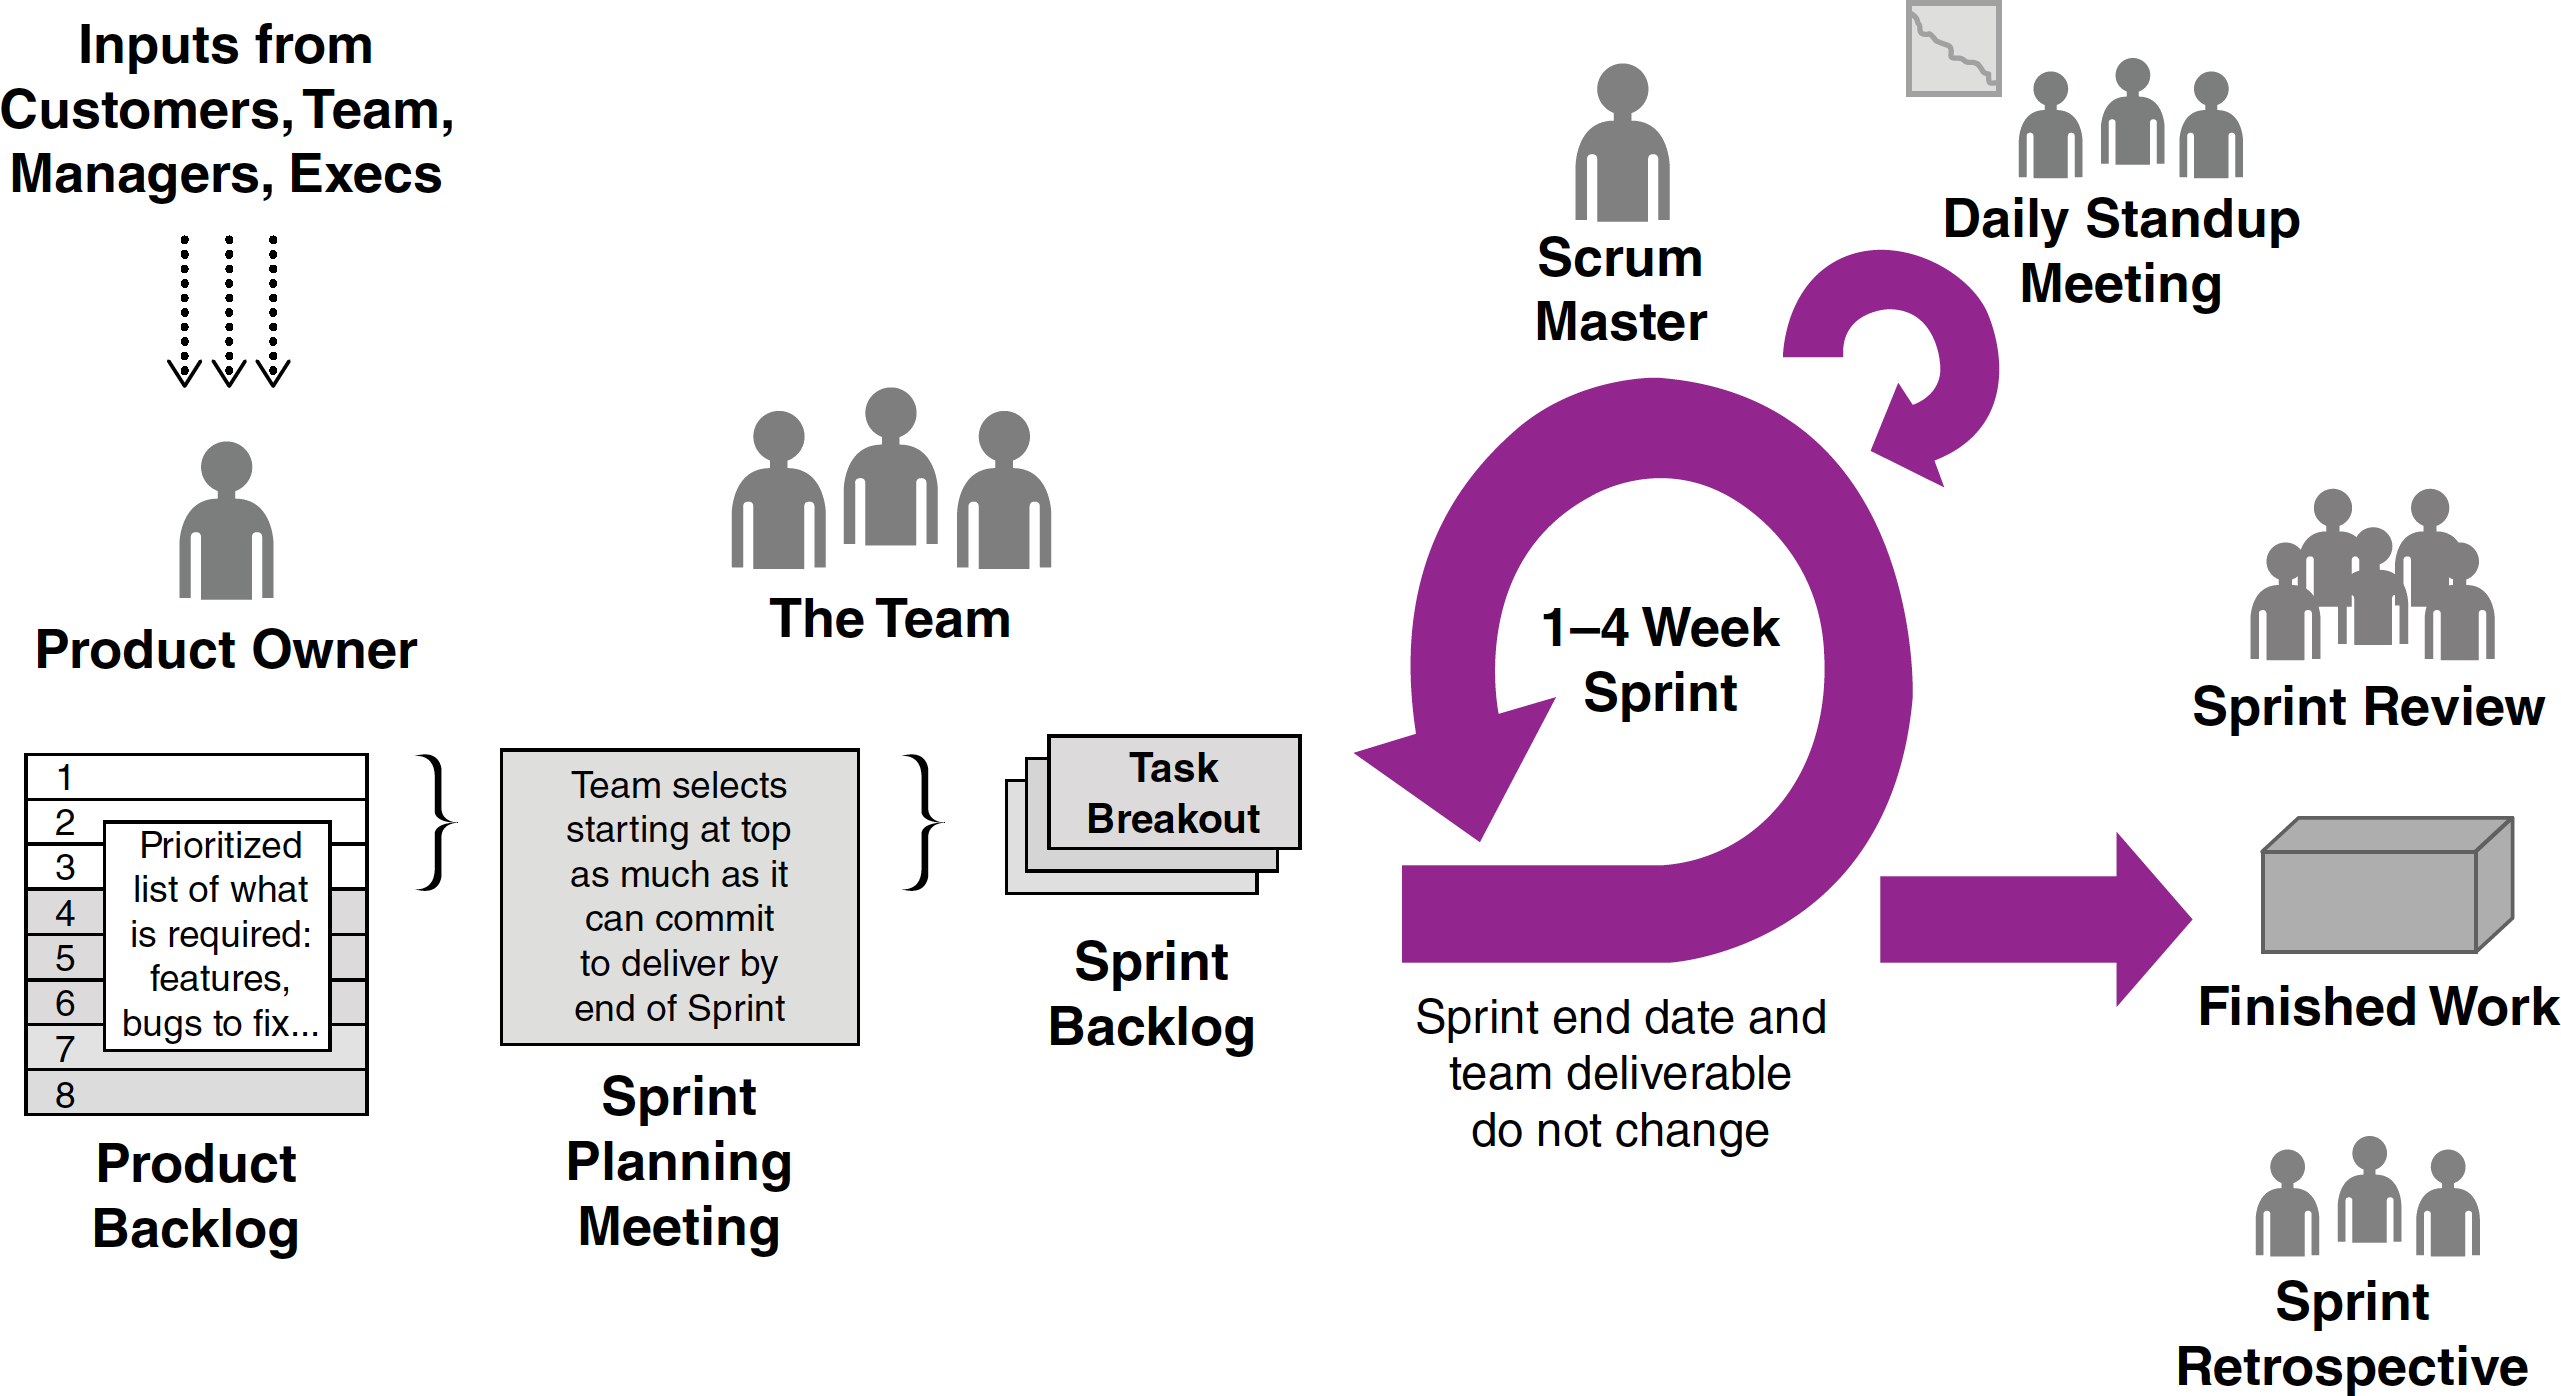
\includegraphics[width=125mm,scale=1]{Figuras/flujo_scrum}
% \caption{Flujo de la técnica SCRUM.}
%   \label{flujo_scrum}
% \end{figure}

\subsection{Planificación de iteraciones}
El primer día de la iteración se realiza la reunión de planificación de la iteración y consta de dos partes:
\begin{itemize}
    \item \textbf{Selección de requisitos} (4 horas máximo) – El PO presenta al equipo la lista de requisitos priorizada del producto o proyecto. El equipo pregunta al PO las dudas que surgen y selecciona los requisitos prioritarios que se compromete a completar en la iteración, de manera que puedan ser entregados en caso de ser solicitados.
    \item \textbf{Planificación de la iteración o sprint} (4 horas máximo) – El equipo elabora la lista de tareas de la iteración necesarias para desarrollar los requisitos a que se ha comprometido. La estimación de esfuerzo se hace de manera conjunta y los miembros del equipo se asignan las tareas.
\end{itemize}

\subsection{Ejecución del Sprint}
El equipo realiza una reunión diaria (15 minutos aproximadamente). Cada miembro del equipo inspecciona el trabajo que el resto está realizando (dependencias entre tareas, progreso hacia el objetivo de la iteración, obstáculos que pueden impedir este objetivo) para poder hacer las adaptaciones necesarias que permitan cumplir con el compromiso adquirido. En la reunión cada miembro del equipo responde a tres preguntas:
\begin{itemize}
    \item ¿Qué he hecho desde la última reunión diaria?
    \item ¿Qué voy a hacer a partir de este momento?
    \item ¿Qué impedimentos tengo o voy a tener?
\end{itemize}
Durante la iteración el Scrum Master se encarga de que el equipo pueda cumplir con su compromiso y de que no se merme la productividad del equipo. Además, elimina los obstáculos que el equipo no puede resolver por sí mismo.

Durante el sprint, el PO junto con el equipo refinen la lista de requisitos para prepararlos para los siguientes sprints y, si es necesario, cambian o vuelven a planificar los objetivos del proyecto para maximizar la utilidad de lo que se desarrolla y el retorno de inversión.

\subsection{Aporte}
En la tabla \ref{mis-aportes} se pueden apreciar los aportes propios en cada historia de usuario. El trabajo consistía en desarrollo de la historia, desarrollo de tests, y el miembro del equipo que no estuvo presente en el desarrollo de la historia es el encargado de hacer la validación de código y funcionalidad.

\begin{table}[H]
\centering
\small
\begin{tabular}{@{}ll@{}}
\toprule
Historias de usuario                                & Aporte \\ \midrule
Diseño de modelo de versionamiento de entidades     &  20\%  \\
Versionamiento de competencias                      & 61,5\% \\
Flujo de trabajo simple                             & 62,5\% \\
Aprobar pasos completados de flujos de trabajo      &  40\%  \\
Rechazar pasos completados de flujo de trabajo      &  60\%  \\
Buzón de entradas de flujos de trabajo              &  40\%  \\
Notificaciones con soporte a etapas                 &  20\%  \\
Versionamiento de evaluaciones                      & 37,5\% \\
Versionamiento de cursos                            & 61,5\% \\
Información básica de curso                         &  20\%  \\
Horas y unidades de evaluación de curso             &   8\%  \\
Especificaciones de curso                           &  40\%  \\
Requisitos de cursos                                &  60\%  \\
Revisar y aprobar curso                             &  40\%  \\
Competencias de curso                               &  25\%  \\
Esquema de curso                                    &  20\%  \\
Códigos de clasificación de curso                   &  60\%  \\
Información básica del programa                     &  50\%  \\
Competencias de programa                            &  60\%  \\
Bloques de curso por programa                       &  20\%  \\
Visualizar cambios en los campos                    &   8\%  \\
Roles de creación y edición para partes             &  23\%  \\
Diseño e implementación de etapas                   &  38\%  \\
Mejora en comportamientos para las etapas por roles & 37,5\% \\
Composición de etapas por roles                     &  23\%  \\
Etapas y partes opcionales por en la revisión       & 37,5\% \\
Notificaciones para las partes de flujos de trabajo &  20\%  \\
Reporte de esquemas de curso                        &  25\%  \\
Interfaz de alineación de códigos TOP/CIP           & 100\%  \\
Reorganización de pestañas del módulo curricular    & 100\%  \\
Lista mejorada de cursos y programas                & 100\%  \\
Retoques finales para el flujo de trabajo de curso  & 37,5\% \\ \bottomrule
\end{tabular}
\caption{Tabla de historias de usuario y aportes}
\label{mis-aportes}
\end{table}

Dichas historias de usuario eran entregadas para validación de parte del equipo de desarrolladores y por el equipo de expertos en didáctica, una vez que era aprobada se procedía a integrar el nuevo código en el repositorio.

\subsection{Inspección y adaptación}
El último día de la iteración se realiza la reunión de revisión del sprint la cual consta de dos partes:
\begin{itemize}
    \item \textbf{Demostración} (3 horas aproximadamente) – El equipo presenta al PO los requisitos completados en la iteración, en forma de incremento de producto preparado para ser entregado con el mínimo esfuerzo. En función de los resultados mostrados y de los cambios ocurridos en el contexto del proyecto, el PO realiza las adaptaciones necesarias de manera objetiva, ya desde la primera iteración, volviendo a planificar el proyecto.
    \item \textbf{Retrospectiva} (1 hora) - El equipo analiza cómo ha sido su manera de trabajar y cuáles son los problemas que podrían impedirle progresar adecuadamente, mejorando de manera continua su productividad. El Scrum Master se encargará de ir eliminando los obstáculos identificados.
\end{itemize}
\section{Validación del desarrollo}

El flujo de validación de las historias de usuario fue un proceso sistemático, consistente y controlado por parte de los desarrolladores y de los expertos en educación encargados de validar el software desarrollado. Las pruebas y otras validaciones abarcan las siguientes dimensiones:
\begin{itemize}
	\item Entradas, salidas y funciones del módulo curricular.
	\item Todos los requisitos no funcionales con sus respectivas pruebas. Como la utilización de tecnologías como Java, MySQL, Bootstrap, entre otras.
	\item Pruebas de rendimiento, fiabilidad, y tiempos de respuesta.
	\item Pruebas por parte de expertos de dominio.
	\item Verificación en diferentes clientes con diversos navegadores y sistemas operativos.
	\item Límites de intervalos, valores por defecto y valores específicos que el módulo acepta.
	\item Criterios de aceptación, especificaciones de requerimientos, funcionales y no funcionales expresados en las historias de usuario y otros documentos del proyecto.
\end{itemize}

Cabe resaltar que la documentación de los casos de prueba en Scrum no involucra necesariamente una secuencia paso a paso a ser utilizada en las pruebas y otros controles de calidad. Al mismo tiempo, los usuarios que validan las historias (expertos en educación en el marco de este proyecto), tienen amplia libertad para aceptar o rechazar las historias de usuarios entregadas por el equipo de desarrollo. 

Así también, los expertos de dominio tienen la potestad de pedir cambios a partir de la experiencia de utilización de las herramientas desarrolladas. Todos estos preceptos fueron observados en la realización de este trabajo.

En la figura \ref{workflow} se puede apreciar el ciclo de vida de las historias de usuario, donde una vez que es creada pasa al estado de \enquote{TODO}, que quiere decir que está pendiente a ser desarrollada. Una vez que un miembro del equipo de desarrollo comienza una historia o tarea pasa al estado de \enquote{IN PROGRESS} y cuando termina pasa al estado de \enquote{UNDER REVIEW}. 

En dicho estado se revisa la funcionalidad mediante validaciones de parte de los miembros del equipo de desarrollo y de parte del equipo de expertos en dominios de didáctica en universidades norteamericanas incluyendo a un PhD en educación, donde se deben cumplir los criterios de aceptación para que pase al estado de \enquote{CLOSED} que quiere decir que se terminó y que la historia fué aprobada.  

En caso de que la historia no consiga cumplir los criterios de aceptación correspondientes durante la validación se considera que la historia no está terminada y que debe pasar al estado de \enquote{REOPEN}, en este estado se puede pasar ya sea desde el estado \enquote{UNDER REVIEW} o si ya está en el estado \enquote{CLOSED}.

Cualquier otro problema o error de código que tenga la nueva funcionalidad se debe crear un ticket de error o bug especificando como reproducir el problema y el comportamiento esperado. En caso de no poder reproducir este comportamiento se pide más información al respecto o pasa al estado de \enquote{CLOSED} en caso de que el comportamiento ya no se pueda reproducir.

\begin{figure}[]
\centering
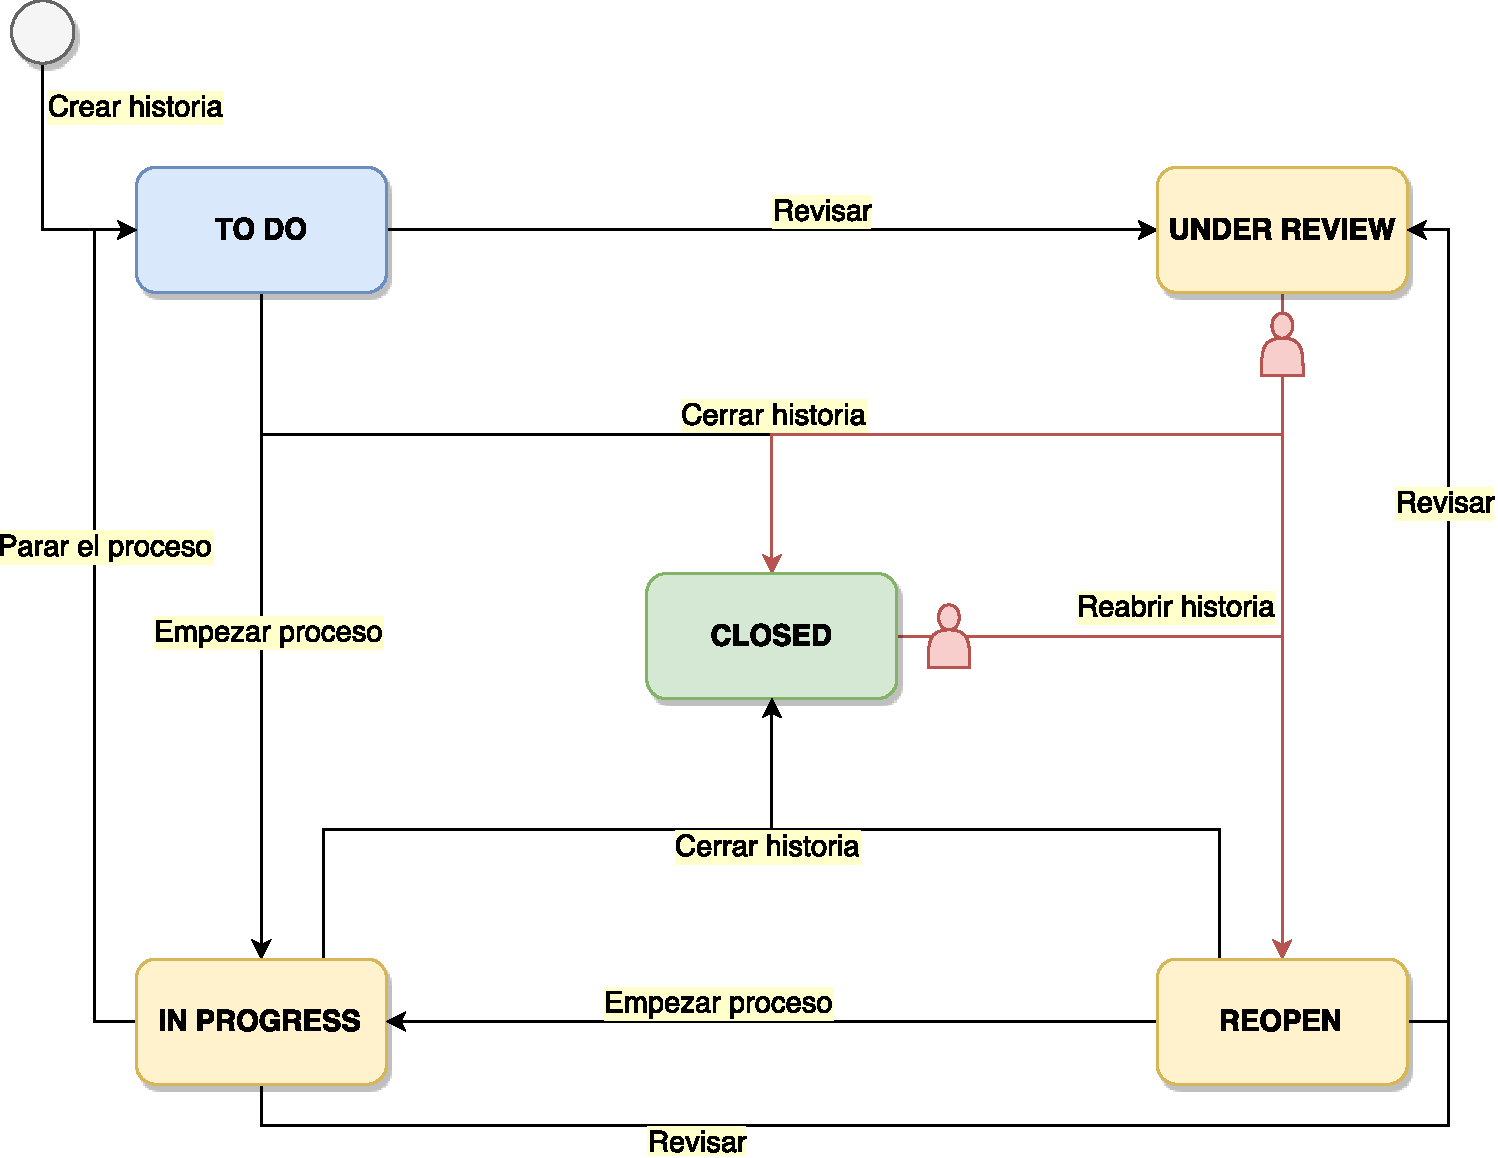
\includegraphics[scale=0.4]{img/workflow}
\caption{Flujo de desarrollo de historias de usuario.}
  \label{workflow}
\end{figure}

\subsection{Revisión por pares}
Revisión por pares significa que los miembros del equipo de desarrollo revisa el código del otro miembro.

El equipo de desarrollo puede realizar evaluaciones por pares durante el desarrollo. La forma en que están sentados puede facilitar este proceso ya que puede dirigirse a la persona que está a su lado y pedirle que revise su trabajo. El equipo de desarrollo también puede reservar tiempo durante el día específicamente para revisar el código. Los equipos autogestionarios deben decidir qué es lo que funciona mejor para su equipo ya sea al inicio de cada iteración o luego de cierto periodo de pruebas.

Por cada funcionalidad terminada y aún en estado \enquote{In Progress} se procede a crear un PR\footnote{de sus siglas en inglés, Pull Request, que es una petición que el propietario de una rama del repositorio hace al propietario del repositorio original para que incorpore los commits que están en la rama.} desde la página de \enquote{GitHub}. 

La plantilla de los PR del repositorio tienen los siguientes campos:
\begin{itemize}
	\item \textbf{Descripción:} se describen los cambios en detalle, ya sea una nueva funcionalidad para el módulo o el problema, causa y cómo se arreglo una falla.
	\item \textbf{Pasos de prueba:} se describe de manera detallada los pasos que se siguieron para probar la rama. Por ejemplo, se coloca el usuario con el rol y cuáles fue la interacción del mismo con la aplicación.
	\item \textbf{Tipo de cambio:} si es una nueva funcionalidad, falla o cambio urgente al sistema.
	\item \textbf{Aceptación de términos y condiciones:} afirmando que se siguió la guía de buenas prácticas de código y que se leyó el documento con las reglas internas de escritura de código. Además, afirmando que las pruebas automatizadas nuevas y existentes pasan.
\end{itemize}

Y deben seguir los siguientes requisitos:
\begin{itemize}
	\item La rama debe estar probada desde una de las instancias del equipo en AWS. En caso de que las pruebas pasan, el usuario que no trabajó en la rama y que se encarga de probar la misma debe aprobar el PR desde la interfaz de revisión de \enquote{GitHub}.
	\item Se deben cumplir los criterios de aceptación y no debe agregar fallas al proyecto. En caso de encontrar fallas se debe notificar al propietario de la rama mediante comentarios desde la interfaz.
	\item Por cada rama en PR se ejecutan las pruebas automatizadas de karma.
	\item Debe pasar las reglas de código estático de la herramienta \enquote{Sonarqube}.
\end{itemize}

En caso de que uno de estos requisitos no se cumplan, \enquote{GitHub} no permite a los usuarios hacer la integración de la rama en el repositorio.

\subsection{Pruebas automatizadas}
Consiste en la automatización de pruebas por medio de código ejecutable, que permite controlar la ejecución de pruebas y la comparación entre los resultados obtenidos y esperados. Las pruebas automatizadas permiten incluir pruebas repetitivas y necesarias dentro de un ciclo de desarrollo para optimizar tiempo utilizado en pruebas manuales\citep{crispin2009agile}.

A menudo, el equipo de desarrollo desarrolla el código durante el día y corren las pruebas automatizadas durante la noche para tener los resultados a la mañana. Por la mañana, el equipo del proyecto puede revisar el informe de errores que generó el programa de pruebas, informar sobre cualquier problema durante el informe diario de cada desarrollador y buscar corregir esos problemas inmediatamente durante el día.

Algunas de las pruebas utilizadas son:
\begin{itemize}
	\item \textbf{Pruebas de integración:} 264 pruebas automatizadas de karma escritas para el módulo curricular, en la cual debían pasar las que hay en el sistema con las nuevas que se agregan.
	\item \textbf{Pruebas de exploración:} con el fin de asegurar la funcionalidad y la estabilidad del producto haciendo pruebas manuales buscando un comportamiento semejante a lo que haría un usuario normal.
	\item \textbf{Análisis de código estático:} 1221 reglas de Java de \enquote{Sonarqube} donde se informa sobre código duplicado, estándares de codificación, potenciales errores, comentarios y diseño del software.
\end{itemize}

Esto permitió comprobar que la aplicación funciona sobre los motores de javascript que la van a ejecutar, lo que nos ayudó a detectar posibles problemas por incompatibilidades de javascript entre ellos.

Con karma para las pruebas de interfaz, se decidió también el uso de la herramienta \enquote{Sonarqube} para evaluar el código fuente que se escribe para el módulo curricular. Donde dicha plataforma utiliza diversas herramientas de análisis estático de código funte para obtener métricas que pueden ayudar a mejorar la calidad del código del programa. Como ya se comentó, uno de los requisitos para que la funcionalidad pueda ser agregada al repositorio es que el PR pase las reglas que la plataforma impone.

\subsection{Revisión por parte del equipo de validación}
Una vez finalizado el proceso de desarrollo y verificación de las historias de usuario, el equipo de validación se encarga de revisar la funcionalidad y verifica que cumple con los criterios de aceptación. El equipo de validación forma parte del ciclo de vida de cada historia de usuario y hace las verificaciones acorde se agreguen a su lista de trabajos pendientes.

Finalmente, el propietario del producto debe comprobar y verificar que la historia de usuario en cuestión cumple con la definición de \enquote{DONE}. Cuando una historia de usuario cumple la definición de \enquote{DONE}, el propietario del producto actualiza la tabla de tareas moviendo la historia de usuario de la columna \enquote{UNDER REVIEW} a la columna \enquote{DONE}.

Por lo general, una vez que el sprint termina, se hace una revisión de las funcionalidades agregadas mediante una reunión utilizando la herramienta \enquote{GoToMeeting}, la cual sirve para reuniones desde cualquier parte del mundo con la capacidad de interactuar y compartir pantallas. El equipo de desarrollo muestra las nuevas funcionalidades y como se acceden a las mismas para facilitar la validación de parte del equipo experto en didáctica. Todos los errores o cambios pequeños de las historias se arreglan luego de la reunión o en caso de que sea muy grande y tome más de un día en arreglarse se procede a la creación de tickets de fallas.

Una vez finalizada la reunión, el equipo de validación y el equipo de desarrollo se comunican a través de la plataforma \enquote{Slack}, donde la misma permite compartir cualquier tipo de archivos, pantallas, y mantener una conversación accediendo desde cualquier plataforma. En la misma plataforma el equipo de validación hace sus consultas y reporta los errores antes de que cree tickets de falla en la plataforma \enquote{JIRA}.
% Chapter 8

\section{Conclusión y aportes}

\subsection{Conclusiones generales}
En el proyecto final se planteó como un caso de estudio con enfoque en la interacción humano-computador a través de una observación participante en el diseño e implementación de un módulo de gestión curricular para un sistema de gestión de evaluaciones basadas en competencias académicas. Se contó con un grupo de expertos en educación así como un grupo de usuarios que acompañaron todo el proceso de desarrollo y validación.

Se diseñó la manera de integrar y estructurar procesos separados de validación de cursos y programas para el estado de California con un sistema de gestión de evaluaciones basadas en competencias. Dicho proceso se realizaba en el pasado en papel y tenía sus falencias debido a que el mismo requería mucho tiempo en revisar y aprobar los formularios pertinentes. Asimismo, la complejidad del flujo aumentaba cuando habían más personas colaboradoras o evaluadoras en el proceso.

Debido a que los requerimientos eran cambiantes y el equipo que diseñaba no disponía de un panorama completo de las funcionalidades del módulo curricular, la elección de la metodología ágil para el desarrollo del proyecto fue acertada debido a que la misma permitía el desarrollo iterativo e incremental del software con validaciones del cliente como proceso de desarrollo, que en este caso el equipo de validación tomaba el rol de cliente debido al conocimiento y experiencia en didáctica de sus miembros.

Por lo tanto, algunas de las experiencias adquiridas en este caso de estudio al utilizar la metodología ágil fueron las siguientes:
\begin{itemize}
	\item Se pudo mejorar rápidamente la elección de que construir, pero tuvimos que tener en cuenta las revisiones de los expertos y usuarios que sugirieron cambios para luego realizarlos.
	\item Se realizó un importante esfuerzo en modular las unidades de trabajo en pequeños incrementos.
	\item Con la experiencia que se fue acumulando, el equipo fue progresivamente mejorando la calidad de sus estimaciones respecto al trabajo que se podía realizar en cada sprint.
\end{itemize}

El diseñar los flujos de trabajo para el diseño y revisión de formularios de competencias, cursos, y programas permitió a los profesores encargados y a los evaluadores de dichos formularios seguir el proceso de una manera intuitiva logrando una mejor experiencia de usuario. Esto se puede apreciar en la aceptación de las historias de usuario y la creación de nuevas historias de mejora, propuestas por los usuarios, que a su vez fueron aprobadas. Un ejemplo de estas mejoras fue la generación de mensajes en cada paso para que el usuario pueda acceder en su buzón de entrada en caso de que tuviera trabajo pendiente.

En el desarrollo del módulo se utilizaron muchas de las tecnologías y herramientas que disponía el sistema como requerimiento no funcional de parte de la organización. El uso de estas tablas en común para la funcionalidad de plantillas de flujos de trabajo trajo consigo muchos problemas técnicos, debido a que agregaba complejidad a las mismas y además las pruebas de componentes se convertían en pruebas de regresión debido a la complejidad de la estructura. 

La decisión de utilizar MySQL para guardar el flujo de trabajo y todos sus datos temporales también acarreó muchos problemas técnicos pues la funcionalidad y el estándar de estructuras de datos de cursos tienen cambios constantes. Sin embargo, la naturaleza iterativa del proceso de desarrollo ágil nos permitió identificar estas falencias y corregirlas en el curso del proyecto.

Debido a la capa adicional de comunicaciones con el usuario final personificada por el equipo de Estados Unidos (que en nuestro caso actúa como cliente), la realimentación de valor real o valor aún necesario provisto al usuario final es lenta e implica grandes cambios luego de varios sprints. Sin embargo, dado el gran número de usuarios finales involucrados, el grupo de expertos también ayudó a clasificar y organizar la comunicación con los mismos.

A pesar de todas las falencias de desarrollo, el módulo tuvo resultados positivos por parte de los usuarios finales ya que la herramienta construida automatiza trabajos de validación curricular para las instituciones. Además, al tener comentarios acerca de qué habría que mejorar en la aplicación y con la utilización de la metodología ágil se permitió que se creen nuevas historias de usuario para algunos retoques futuros en el módulo curricular. 

\subsection{Aportes del proyecto}
La capacidad otorgada por este sistema para gestionar el diseño y validación de material curricular en el estado de California, y la comunicación que ofrece entre los encargados del diseño de los formularios y los evaluadores de los mismos constituye el principal aporte de este trabajo.

Además, podemos citar otros aportes:
\begin{itemize}
	\item El módulo desarrollado reemplaza la preparación manual de formularios, los procesos de revisión y aprobación curricular de colegios ya sea para universidades, cursos, y programas.
	\item El módulo constituye un ambiente que puede ser accedido desde cualquier navegador y la capacidad de compartir comentarios, permite a las personas trabajar en conjunto sin necesidad de agendar reuniones para desarrollar el formulario o las revisiones.
	\item El módulo desarrollado permite almacenar los datos nuevos, históricos, propuestos y activos de competencias, cursos, y programas.
	\item Al proveer notificaciones automatizadas cuando hay cambios de estado en los flujos de trabajo.
	\item En la opinión de expertos y usuarios, la utilización del módulo desarrollado reduciría el tiempo promedio de formulación y revisión de cada flujo de diseño e implementación de flujos de trabajo, debido a que el mismo facilita la labor de llenar formularios utilizando información ya existente en el AMS.
\end{itemize}


\subsection{Trabajos futuros}
En consenso con los usuarios finales de la aplicación y los que diseñan las historias de usuarios se observaron ciertas características que podrían dar una mayor utilidad al proyecto, donde citaremos algunos de los trabajos futuros ya creadas como épicas del proyecto:
\begin{itemize}
	\item \textbf{Importador de cursos:} muchos de los cursos que ya fueron agregados al sistema de gestión curricular del estado de California existen y como trabajo futuro para el módulo curricular es la forma de importar todos estos cursos al AMS sin necesidad de hacer todo el flujo de trabajo para las competencias, cursos y programas válidos actualmente.
	\item \textbf{Migración de motor de base de datos de los flujos de trabajo:} como ya comentamos, la decisión de tecnología en cuanto al motor de base de datos fue una decisión errónea, debido a que el estándar de California para diseño y revisión de cursos y programas puede variar con el tiempo y la utilización de MySQL como motor de base de datos dificulta el desarrollo en sí debido al constante cambio del modelo de datos, por lo que se considera un motor de base de datos no relacional basada en documentos, e.g. \enquote{MongoDB} como una opción a futuro.
	\item \textbf{Acceso de información a través de API\footnote{de sus siglas en inglés, Application Programming Interface, que sirve como un conjunto de reglas para que las aplicaciones puedan comunicarse entre ellas.} pública:} es una práctica que exige el estado de California que todos los datos en cuanto a cursos y programas de las universidades puedan ser accedidas desde una API pública. Por lo tanto, se debe diseñar e implementar una interfaz pública que permita comunicarse y acceder a los datos del módulo curricular.
	\item \textbf{Catálogo de cursos:} los CMS del estado tienen la opción de mostrar sus cursos válidos de manera pública para que las universidades puedan cargar en sus sistemas académicos como se aprecia en la figura \ref{after_creation}. Por lo tanto, como trabajo futuro para el módulo curricular se busca catalogar los cursos de manera pública desde una interfaz web.
	\item \textbf{Flujo de trabajo para evaluaciones:} el mismo flujo de trabajo que se diseño e implementó para las competencias, cursos, y programas, se debe implementar para las evaluaciones.
\end{itemize}
Desde el punto de vista académico sería interesante realizar una experiencia controlada de usabilidad del sistema para medir con mayor precisión las ganancias en materia de productividad que conlleva la utilización de este módulo.

%----------------------------------------------------------------------------------------
%	BIBLIOGRAPHY
%----------------------------------------------------------------------------------------
\printbibliography[heading=bibintoc,title={Bibliografía}]

\end{document}